\section{اصول طراحی چندرسانه‌ای آموزشی}
\label{s:multimedia}
\subsection{اصل انسجام}
یادگیری افراد هنگامی که محتوای فرعی حذف شود افزایش می‌یابد نسبت به زمانی که این محتوا وجود داشته باشد، این اصل را می‌توان به سه بیان دیگر عنوان نمود: ‍(۱) یادگیری هنگامی که تصاویر و کلمات نامربوط هرچند جذاب حذف شوند، افزایش پیدا می‌کند. (۲) یادگیری هنگامی که صداها و موسیقی نامربوط هرچند جذاب حذف شوند، افزایش پیدا می‌کند. (۳) یادگیری هنگامی که کلمه ها و نماد های غیرضروری از آن حذف شود افزایش پیدا می‌کند.
\\
\textbf{مثال}
گروه روایت مختصر: فرد یادگیرنده روایت مختصری از پویانمایی را می‌بیند.
گروه روایت اضافی: فرد یادگیرنده همان درس را با فیلم‌ها، موسیقی، جزئیات، اطلاعات نامربوط و تصاویر می‌بیند. در تصویر 
\ref{fig:coherenceexample}
می‌توانید نمونه ای از آن را ببینید.
\\
محتوای اضافه می‌تواند منابع شناختی فرد یادگیرنده را مورد استفاده قرار دهد در نتیجه منابع کمتری به محتوای اصلی خواهد رسید، از این رو توجه فرد کمتر خواهد شد و فرایند یادگیری او دچار اختلال می‌شود. این اصل به ویژه زمانی نقش کلیدی پیدا می‌کند که ظرفیت حافظه کاری و دانش اش کمتر باشد.
روی دیگر حالتی است که فرد در زمینه مورد یادگیری با تجربه باشد، در این حالت ممکن است این اصل صدق نکند و مؤثر نباشد، به بیان دیگر اضافه کردن جزئیات آموزش برای افرادی که تازه موضوعی را یاد می‌گیرند مناسب نباشد ولی به یادگیری افراد با تجربه کمک کند. با رعایت این اصل و حذف محتوای غیرضروری به مفید و مختصر شدن محتوای آموزشی کمک خواهد شد.
\cite{mayer2009multimedia}
این اصل در ۲۲ آزمایش از ۲۳ آزمایش تجربی تایید شده است. به طور مثال در یک آزمایش دو متحوای چند رسانه ای در رابطه با نحوه پخش ویروس ها تهیه شده بود، اولی با محتوای فرعی(جملاتی که حقایق جالب ولی بدون ارتباط به ویروس ها را بیان می‌کرد) و دیگری تنها اصل متحوی نتایج نشان داد گروهی که محتوای دوم را دیده بودند عملکرد بهتری نسبت به گروه اول داشتند.
\cite{mayer2008increased}

\begin{figure}[htbp]
	\centering
	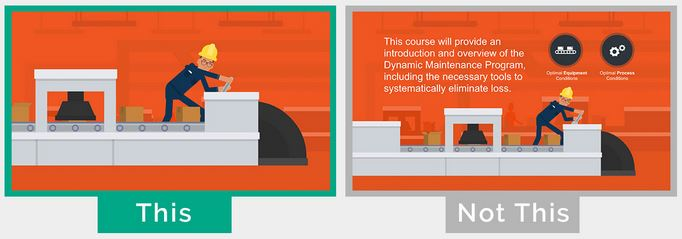
\includegraphics[width=0.7\linewidth]{figures/Coherence_example}
	\caption[مثال اصل انسجام]{مطابق اصل انسجام تمامی موارد اضافی را حدف کنید و از تصاویر و کلمات ساده که مستقیما در ارتباط با آموزش است استفاده کنید که به یادگیری فرد کمک کند
	\cite{principle_examples}}
	\label{fig:coherenceexample}
\end{figure}


\subsection{اصل نشانه گذاری}
هنگامی که ساختار محتوای اصلی یک چندرسانه‌ای نشانه گذاری شده باشد افراد بهتر یاد می‌گیرند. همچنین نشانی گذاری می‌تواند در محتواهایی که دارای عناصر فرعی هستند و یا هنگامی که فرد توانایی خواندن بالایی ندارد کمک کننده باشد. منتقدان این اصل می‌گویند نشانه گذاری محتوایی به چندرسانه‌ای اضافه نمي کند و موجب افزونگي مي شود از اين رو فرايند يادگيري را مختل مي کند.
\\
می‌توان نشانه گذاری را به دو بخش تقسیم نمود:
\begin{enumerate}
\item
\textit{نشانه گذاری دیداری}
مثل کم رنگ کردن بخشی از محتوا، رنگ‌های متمایز، چشمک زدن، جهت نماها و حرکات اشاره گر
\item
\textit{نشانه گذاری کلامی}
مثل تاکید آوایی، کلمات اشاره‌گر،‌سرفصل ها و طرح کلی
\end{enumerate}
از دیگر مزیت های نشانه گذاری هنگامی است که محتوای چندرسانه‌ای دارای بار فرعی باشد، نشانه گذاری با جلب توجه یادگیرنده به محتوای اصلی سبب خواهد شد تا فرایند یادگیری دچار اختلال نشود.

\textbf{مثال}
در یک پویانمایی که سیارات منظومه شمسی را نشان می‌دهد نشانه گذاری، شامل افزودن نام سیارات و تاکید کلامی برای آن‌ها می‌باشد.

این اصل توسط ۲۵ آزمایش از ۲۹ آزمایش تجربی تایید شده است. مایر در تحقیق‌های خود شواهدی بر اثر بخش تر بودن نشانه گذاری دیداری نسبت نشانه گذاری کلامی مشاهده کرد همچنین برخی مشاهد‌‌ه‌ها نشان می‌دهند استفاده بیش از حد از نشانه گذاری‌ سبب زیان دیدن فرایند یادگیری خواهد شد.
در تصویر
\ref{fig:signalingexample}
می توانید مثالی از این اصل ببینید.
\begin{figure}[htbp]
	\centering
	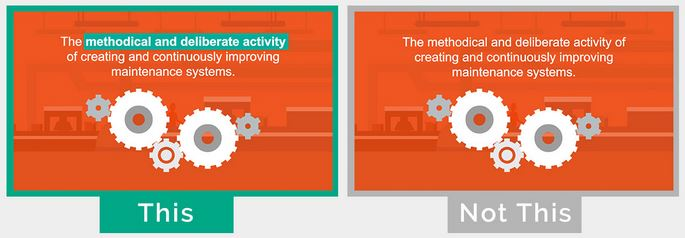
\includegraphics[width=0.7\linewidth]{figures/Signaling_example}
	\caption[مثال اصل نشانه گذاری]{به یادگیرنده دقیقا نشان دهید چه چیزی مهم است. با قرار دادن فلش و یا برجسته کردن می‌توانید نکات و لغات مهم را نشان دهید}
	\label{fig:signalingexample}
\end{figure}

\subsection{اصل افزونگی}
افراد از گرافیک و روایت نسبت به گرافیک، روایت و متن چاپ شده بهتر یاد می‌گیرند.
\\
\textbf{مثال}
گروه دارای افزونگی: به افراد فیلمی از نحوه تشکیل رعد و برق نشان داده می‌شود هم‌زمان همان متن روایت شده زیر نویس می‌شود.
\\
گروه بدون افزونگی: به این گروه همان فیلم ولی بدون زیر نویس نشان داده می‌شود. در تصویر
\ref{fig:redundancyexample}
ميتوانید مثال این اصل را ببینید.
\\ 
افزونگی باعث ایجاد پردازش فرعی می‌شود، زیرا کانال بصری زمانی که باید به محتوای اصلی توجه کند دچار سربار می‌شود همچنین، یادگیرندگان برای مقایسه روایت و متن نمایش داده شده تلاش ذهنی دارند. با این حال اگر (الف) متن نمایش داده شده محدود به لغات کمی باشد و پس روایت نمایش داده شود (ب) بجای همزمان بودن روایت و نمایش متن، متن پیش از روایت نمایش داده شود. (ج) بخش های کلامی کوتاه شوند و گرافیک به کار نرود، در هر یک از این سه مورد بار فرعی کاهش پیدا می‌کند.
\\
فرضیه‌ای وجود دارد که می‌گوید: افراد متفاوت از راه‌های متفاوت یاد می‌گیرند، پس بهترین راه این است که اطلاعات را در قالب های مختلف زیادی ارائه کنیم. به این فرضیه ترجیحات یادگیری
\LTRfootnote{Learning preferences hypothesis}
 گویند.
 به عنوان مثال محتوایی ایجاد کرد که هم دارای روایت و هم متن باشد،‌ حال دانش آموزی که ترجیح می‌دهد با صدای کلمات یاد بگیرید، می تواند به روایت توجه کند و دیگری که ترجیح می دهد کلمات نوشته شده را بخواند می‌تواند به متن نمایش داده شده توجه کند. با این روش آموزگاران می توانند سبک یادگیری
 \LTRfootnote{Learning Style}
 هر دانش آموز را پوشش دهند.
 \\
 هنگامی که پویانمایی و متن روی صحفه همزمان باشند، حافظه کاری دچار سربار می‌شود که نشان می‌دهد اصل افزونگی با فرضیه محدودیت ظرفیت سازگار است. برخی پژوهش ها نیز نشان می‌دهند که هنگامی که پویانمایی با سرعت بالا نمایش داده می‌شود بهتر است که متن نمایش داده شده دقیقا همان متن روایت شده نباشد بهتر است.
 راهکار های  مفید می‌تواند شامل این موارد باشد: نوشتن نکات کلیدی بر روی تخته، نوشتن متن های شامل اصطلاح‌های‌ فنی و ناآشنا و یا هنگامی متن کتاب طولانی و پیچیده باشد.
\begin{figure}[htbp]
	\centering
	
\includegraphics[width=0.7\linewidth]{figures/Redundancy_example}
	\caption[مثال اصل افزونگی]{هنگامی که یک روایت همراه با گفتار پخش می‌شود تنها از تصاویر استفاده کنید نه از تصویر و متن این اجازه را به کاربر بدهید تا به صورت دلخواه بتواند متن زیر نویس را فعال و یا غیرفعال کند}
	\label{fig:redundancyexample}
\end{figure}

\subsection{اصل مجاورت مکانی}
اصل مجاورت مکانی
\LTRfootnote{Spatial contiguity principle}
می‌گوید: اگر تصاویر و کلمات مربوط به هم به یکدگیر نزدیک باشند دانش آموزان بهتر یاد می‌گیرند تا حالتی که از هم دور باشند.
\\
\textbf{مثال}
در پویانمایی ای که نحوه شکل گیری رعد و برق را نمایش می‌دهد کلمات در پایین صحفه نمایش داده می‌شوند، (پویا نمایی جدا از هم) و یا اینکه کلمات در کنار رویدادی که دراند توضیح می‌دهند قرار بگیرند. (پویا نمایی نزدیک به هم)، البته همین مثال را می‌توان برای جزوه هم در نظر گرفت که کلمات نزدیک به تصویر باشند و یا دور از آن. در تصویر
\ref{fig:spatialexample}
مثالی از این اصل را می‌بینید.
\\
در حالتی که کلمات به تصویری که توضیح می‌دهند نزدیک باشند، یادگیرنده منابع شناختی کمتری برای یافتن آنها صرف خواهد نمود.  این اصل در مواردی مثل: یادگیرنده با محتوا آشنایی ندارد، نمودارها بدون متن هستند و به طور کامل قابل فهم نیستند و یا زمانی که محتوا پیچیده تر باشد کاربرد بیشتری دارد. 
\\
در تمامی ۵ آزمایش گرفته شده از دانش آموزان، گروهی که کلمات و تصاویر متناظر در کنار یکدیگر بوده اند نسبت به گروه دیگر که کلمات و تصاویر متناظر دور از یکدیگر بوده اند عملکرد بهتری داشته اند.
\\
موارد بحثی در این زمنیه وجود دارد، مخالفان می گویند، نمایشن همزمان متن و تصویر نزدیک به هم که یک معنا را می‌رسانند سبب ایجاد بار اضافی برای فرد یادگیرنده شده و منابع شناختی او را مصرف می‌کنند، از طرفی از نظر موافقان تطابق میان کلمات و تصاویر سبب صرف منابع شناختی جهت یادگیری فعال خواد بود.
\\
پژوهش‌های آینده می‌تواند حول این موارد باشد، نقش دانش قبلی یادگیرنده و میزان کاهش دادن اثر طراحی ضعیف توسط این دانش، روش هایی برای اندازه گیری دانش قبلی، تعداد لغات مورد نیاز جهت قرار گرفتن در کنار تصویر و در نهایت این اصل ممکن با اصل کیفیت در تضاد باشد، پس باید پژوهش هایی انجام شود تا بفهمیم چه هنگام از متن و چه هنگام از گفتار برای یک تصویر استفاده کنیم.
\begin{figure}[htbp]
	\centering
	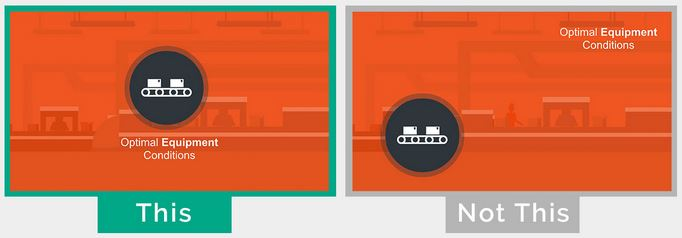
\includegraphics[width=0.7\linewidth]{figures/spatial_example}
	\caption[مثال اصل مجاورت مکانی]{تمامی متن ها و تصاویر مرتبط در یک قاب را به یکدیگر نزدیک نگهدارید. با اینکار یادگیرندگان ارتباط میان مفاهیم را راحت تر در می‌یابند.}
	\label{fig:spatialexample}
\end{figure}

\subsection{اصل مجاورت زمانی}
اصل مجاورت زمانی
\LTRfootnote{Temporal Contiguity Principle}
می‌گوید: هنگامی که تصاویر و کلمات به صورت همزمان نمایش داده شوند، دانش آموزان بهتر یاد می‌گیرند تا حالتی که پیوسته نمایش داده شوند.
\\
\textbf{مثال}
یادگیرندگان اول پویانمایی ای از نحوه شکل گیری رعد و برق می بینند و سپس می‌شنوند روایت آن را و یا با یک ترتیب دیگر(گروه پیاپی)، و یا یادگیرندگان پویانمایی را می‌بینند و می‌شنوند روایتش را به صورت همزمان (گروه همزمان).
(گروه همزمان) یادگیرندگان پویانمایی از نحوه شکل گیری رعد و برق می بییند، بدین صورت که تصاویر و روایت به صورت همزمان نمایش داده می شود. (گروه پیاپی) در این گروه ابتدا نحوه شکل گیری رعدوبرق را می‌بینند سپس روایت متنظار آن را می‌شنوند و یا برعکس این ترتیب.
\\
هنگامی که روایت و پویانمایی متناظر آن به صورت همزمان ارائه شود،‌ فرد می‌تواند بازنمایی هر دو را به صورت همزمان در ذهن خود نگهدارد، و اتصال‌های ذهنی بهتری را بین بازنمایی کلامی و بصری برقرار کند، و بر عکس آن یعنی زمانی که به صورت غیر همزمان ارائه شوند نیز صدق می‌کند.
\\
این اصل ممکن است در دو حالت کاربرد کمتری داشته باشد: حالت اول زمانی که ارائه و یا درس مورد نظر فرایند پخش و کنترل آن دست یادگیرنده باشد تا زمانی که دست سیستم باشد و حالت دوم زمانی که پویانمایی شامل بخش های کوچک جدا از هم باشد تا زمانی که یک درس طولانی و پیوسته داشته باشیم. زمانی که تصویر و روایت از هم جدا شوند مطابق حس ما که می‌گوید یک مطلب را دوبار ببینیم بهتر یاد می‌گیریم، امکان یادگیری نیز بیشتر می‌شود، در مرحله اول فرد توجه کامل خود را به تصاویر می‌کند و در مرحله بعدی مطالبی که تصاویر آن را دیده به صورت روایت می‌شنود. این تحلیل بر این مبنا است که اگر ما یک محتوا را از دو انتقال،‌ دریافت کنیم شانس بیشتری برای ذخیره سازی در حافظه کاری داریم نسبت به زمانی که تنها یکبار آن را ببینیم.

\subsection{سایر اصول طراحی چندرسانه‌ای آموزشی}
این اصول بر خلاف پنج اصل قبلی که به پیچیدگی رسانه انتقال و طراحی آن به نحوی که این پیچیدگی کاهش پیدا کند به، پیچیدگی ذاتی محتوا و توانایی یادگیرنده در ساخت الگوهای شناختی می پردازند از این رو این اصول را به صورت خلاصه بررسی می کنیم.
\subsubsection{اصل قطعه‌بندی}
مطابق اصل قطعه بندی
\LTRfootnote{Segmenting Principle}
زمانی که محتوای آموزشی بخش بندی شود و کاربرد بتواند خود را با آن همگام کند بهتر یادگرفته می‌شود تا زمانی که تنها یک فیلم پیوسته داشته باشیم.
\subsubsection{اصل پیش‌آموزش}
در اصل پیش آموزش
\LTRfootnote{Pre-training principle}
داریم،‌ هنگامی که افراد پیش از آموزش با نام‌ها و مشخصه‌های مفاهیم اصلی آشنا باشند بهتر یاد می‌گیرند.
\subsubsection{اصل کیفیت}
اصل کیفیت
\LTRfootnote{Modality principle}
می‌گوید، در حالتی که محتوا از طریق تصویر و روایت باشد یادگیری عمیق تری خواهیم داشت تا زمانی که از طریق تصویر و نوشته‌های چاپی باشد.
\subsubsection{اصل چندرسانه‌ای}
مطابق اصل چندرسانه‌ای
\LTRfootnote{Multimedia principle}
، هنگامی که یادگیری از کلمات و تصاویر باشد یادگیری بهتری داریم تا زمانی که تنها از طریق کلمات باشد.
\subsubsection{اصل شخصی‌سازی}
در اصل شخصی‌سازی
\LTRfootnote{Personalization principle}
داریم، اگر روایت و گفتار به صورت غیررسمی باشد افراد بهتر یاد می‌گیرند تا زمانی که رسمی باشد.
\subsubsection{اصل صدا}
اصل صدا
\LTRfootnote{Voice principle}:
افردا از صدای طبیعی بهتر یاد می‌گیرند تا صدای مصنوعی و ماشینی.
\subsubsection{اصل تصویر}
اصل تصویر
\LTRfootnote{Image principle}:
ممکن است یادگیری در زمانی که همزمان با روایت، تصویر آموزگار پخش شود دچار اختلال شود.